\documentclass[12pt]{article}
\usepackage[margin=1in]{geometry}

% Start of preamble
%==========================================================================================%
% Required to support mathematical unicode
\usepackage[warnunknown, fasterrors, mathletters]{ucs}
\usepackage[utf8x]{inputenc}

% Always typeset math in display style
%\everymath{\displaystyle}

% GROUPOIDS FONT!
\usepackage{eulervm}
\usepackage{charter}

% Standard mathematical typesetting packages
\usepackage{amsthm, amsmath, amssymb}
\usepackage{mathtools}  % Extension to amsmath

% Symbol and utility packages
\usepackage{cancel, textcomp}
\usepackage[mathscr]{euscript}
\usepackage[nointegrals]{wasysym}

% Extras
\usepackage{physics}  % Lots of useful shortcuts and macros
\usepackage{tikz-cd}  % For drawing commutative diagrams easily
\usepackage{color}  % Add some color to life
\usepackage{microtype}  % Minature font tweaks
%\usepackage{pgfplots} % plots

\usepackage{enumitem}
\usepackage{titling}

\usepackage{graphicx}

% Common shortcuts
\def\mbb#1{\mathbb{#1}}
\def\mfk#1{\mathfrak{#1}}

\def\bN{\mbb{N}}
\def\bC{\mbb{C}}
\def\bR{\mbb{R}}
\def\bQ{\mbb{Q}}
\def\bZ{\mbb{Z}}

% Sometimes helpful macros
\newcommand{\floor}[1]{\left\lfloor#1\right\rfloor}
\newcommand{\ceil}[1]{\left\lceil#1\right\rceil}
\DeclarePairedDelimiterX\set[1]\lbrace\rbrace{\def\given{\;\delimsize\vert\;}#1}

% Some standard theorem definitions
\newtheorem{theorem}{Theorem}[section]
\newtheorem{corollary}{Corollary}[theorem]
\newtheorem{lemma}[theorem]{Lemma}

\theoremstyle{definition}
\newtheorem{definition}{Definition}[section]

\theoremstyle{remark}
\newtheorem*{remark}{Remark}

% End of preamble
%==========================================================================================%

% Start of commands specific to this file
%==========================================================================================%

\newcommand{\R}{\mathbb{R}}
\renewcommand{\ip}[2]{\langle #1, #2 \rangle}
\newcommand{\mg}[1]{\| #1 \|}
\newcommand{\linf}[1]{\max_{1\leq i \leq #1}}
\newcommand{\ve}{\varepsilon}
\renewcommand{\qed}{\hfill\qedsymbol}
\newcommand{\seq}[2]{\qty(#1_#2)_{#2=1}^{\infty}}
\newcommand\setItemnumber[1]{\setcounter{enumi}{\numexpr#1-1\relax}}
\newcommand{\justif}[1]{&\quad &\text{(#1)}}
\newcommand{\ra}{\rightarrow}


%==========================================================================================%
% End of commands specific to this file

\title{CSE 311 Quiz 9}
\date{\today}
\author{Rohan Mukherjee}

\begin{document}
	\maketitle
	\begin{enumerate}[leftmargin=\labelsep]
		\item \begin{enumerate}
			\item It is not transitive, not reflexive, not symmetric, and vacuously anti-symmetric (there will never be the case where $x = y+1$ and $y = x+1$).
			\item Given an arbitrary $x \in \R$, clearly $x^2=x^2$, so $(x, x) \in S$. Given arbitrary $a, b, c \in \R$, if $(a, b) \in S$, and $(b, c) \in s$, then $a^2=b^2$, and $b^2=c^2$. Because equality is transitive, we see that $a^2=c^2$, which shows that $(a, c) \in S$. Given arbitrary $x, y \in R$, if $(x, y) \in S$, then $x^2=y^2$. Because equality is symmetric, $y^2=x^2$, which shows that $(y, x) \in S$, which means that $S$ is symmetric.
		\end{enumerate}
		\setItemnumber{3}
		\item
		\begin{enumerate}
			\item \begin{align*}
				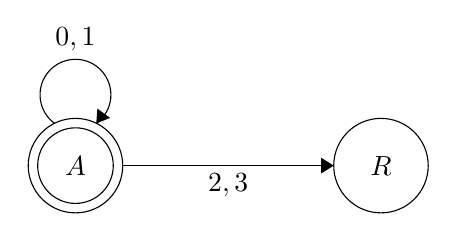
\begin{tikzpicture}[scale=0.2]
					\tikzstyle{every node}+=[inner sep=0pt]
					\draw [black] (26.6,-24) circle (3);
					\draw (26.6,-24) node {$A$};
					\draw [black] (26.6,-24) circle (2.4);
					\draw [black] (46,-24) circle (3);
					\draw (46,-24) node {$R$};
					\draw [black] (25.277,-21.32) arc (234:-54:2.25);
					\draw (26.6,-16.75) node [above] {$0,1$};
					\fill [black] (27.92,-21.32) -- (28.8,-20.97) -- (27.99,-20.38);
					\draw [black] (29.6,-24) -- (43,-24);
					\fill [black] (43,-24) -- (42.2,-23.5) -- (42.2,-24.5);
					\draw (36.3,-24.5) node [below] {$2,3$};
				\end{tikzpicture}
			\end{align*}
			The start arrow should've pointed at A, but I forgot to add it.
			\item 
			\begin{align*}
				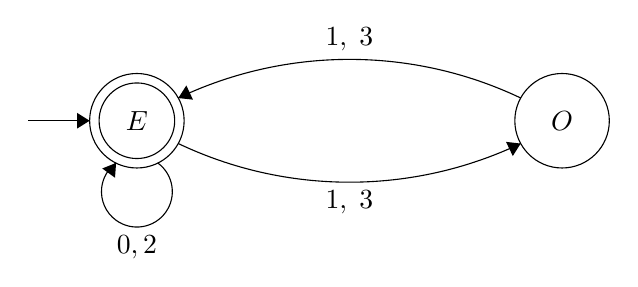
\begin{tikzpicture}[scale=0.2]
					\tikzstyle{every node}+=[inner sep=0pt]
					\draw [black] (13.4,-29) circle (3);
					\draw (13.4,-29) node {$E$};
					\draw [black] (13.4,-29) circle (2.4);
					\draw [black] (40.4,-29) circle (3);
					\draw (40.4,-29) node {$O$};
					\draw [black] (6.5,-29) -- (10.4,-29);
					\fill [black] (10.4,-29) -- (9.6,-28.5) -- (9.6,-29.5);
					\draw [black] (14.723,-31.68) arc (54:-234:2.25);
					\draw (13.4,-36.25) node [below] {$0,2$};
					\fill [black] (12.08,-31.68) -- (11.2,-32.03) -- (12.01,-32.62);
					\draw [black] (37.774,-30.447) arc (-64.54137:-115.45863:25.297);
					\fill [black] (37.77,-30.45) -- (36.84,-30.34) -- (37.27,-31.24);
					\draw (26.9,-33.4) node [below] {$1,\mbox{ }3$};
					\draw [black] (16.027,-27.555) arc (115.41534:64.58466:25.334);
					\fill [black] (16.03,-27.56) -- (16.96,-27.66) -- (16.54,-26.76);
					\draw (26.9,-24.6) node [above] {$1,\mbox{ }3$};
				\end{tikzpicture}
			\end{align*}
			\item 
			\begin{align*}
				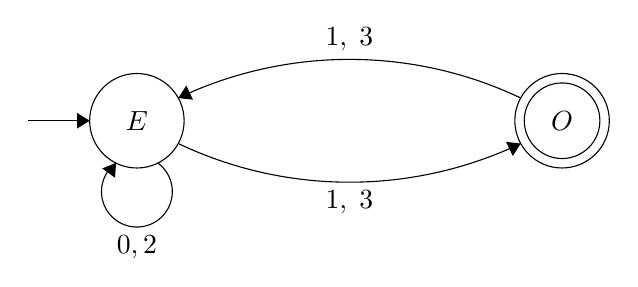
\begin{tikzpicture}[scale=0.2]
					\tikzstyle{every node}+=[inner sep=0pt]
					\draw [black] (13.4,-29) circle (3);
					\draw (13.4,-29) node {$E$};
					\draw [black] (40.4,-29) circle (3);
					\draw (40.4,-29) node {$O$};
					\draw [black] (40.4,-29) circle (2.4);
					\draw [black] (6.5,-29) -- (10.4,-29);
					\fill [black] (10.4,-29) -- (9.6,-28.5) -- (9.6,-29.5);
					\draw [black] (14.723,-31.68) arc (54:-234:2.25);
					\draw (13.4,-36.25) node [below] {$0,2$};
					\fill [black] (12.08,-31.68) -- (11.2,-32.03) -- (12.01,-32.62);
					\draw [black] (37.774,-30.447) arc (-64.54137:-115.45863:25.297);
					\fill [black] (37.77,-30.45) -- (36.84,-30.34) -- (37.27,-31.24);
					\draw (26.9,-33.4) node [below] {$1,\mbox{ }3$};
					\draw [black] (16.027,-27.555) arc (115.41534:64.58466:25.334);
					\fill [black] (16.03,-27.56) -- (16.96,-27.66) -- (16.54,-26.76);
					\draw (26.9,-24.6) node [above] {$1,\mbox{ }3$};
				\end{tikzpicture}
			\end{align*}
			This one was pretty nice. I answered two questions but only had to think one time.
		\end{enumerate}
		\setItemnumber{5}
		\begin{enumerate}
			\item It seems to accept $(0)^*1(0)^*$.
			\item \begin{align*}
				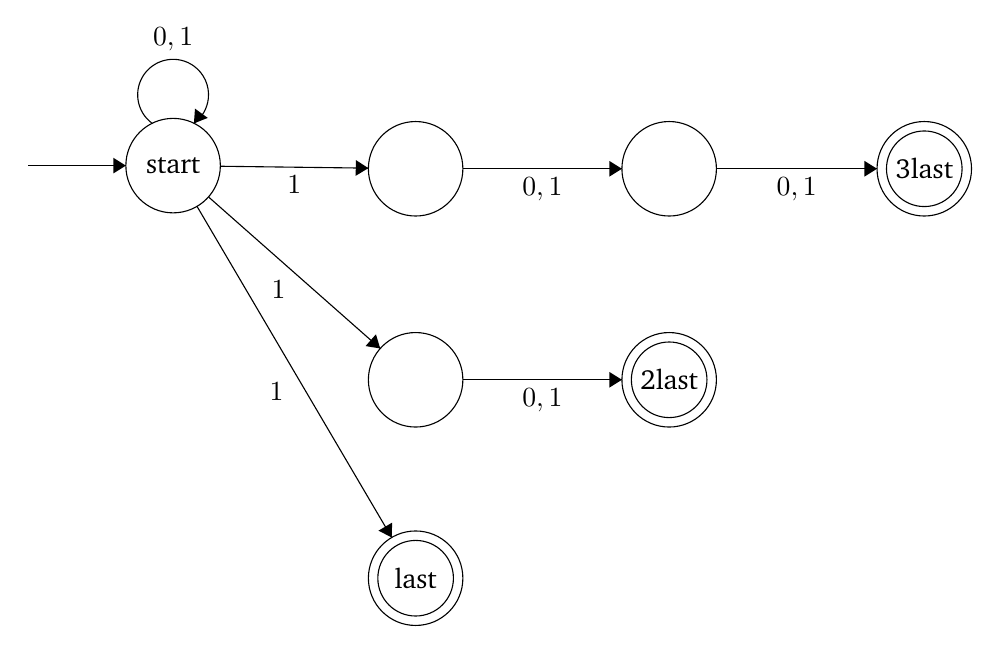
\begin{tikzpicture}[scale=0.2]
					\tikzstyle{every node}+=[inner sep=0pt]
					\draw [black] (14.9,-24.3) circle (3);
					\draw (14.9,-24.3) node {start};
					\draw [black] (30.3,-24.5) circle (3);
					\draw [black] (46.4,-24.5) circle (3);
					\draw [black] (62.6,-24.5) circle (3);
					\draw (62.6,-24.5) node {3last};
					\draw [black] (62.6,-24.5) circle (2.4);
					\draw [black] (30.3,-37.9) circle (3);
					\draw [black] (46.4,-37.9) circle (3);
					\draw (46.4,-37.9) node {2last};
					\draw [black] (46.4,-37.9) circle (2.4);
					\draw [black] (30.3,-50.5) circle (3);
					\draw (30.3,-50.5) node {last};
					\draw [black] (30.3,-50.5) circle (2.4);
					\draw [black] (5.7,-24.3) -- (11.9,-24.3);
					\fill [black] (11.9,-24.3) -- (11.1,-23.8) -- (11.1,-24.8);
					\draw [black] (13.577,-21.62) arc (234:-54:2.25);
					\draw (14.9,-17.05) node [above] {$0,1$};
					\fill [black] (16.22,-21.62) -- (17.1,-21.27) -- (16.29,-20.68);
					\draw [black] (17.9,-24.34) -- (27.3,-24.46);
					\fill [black] (27.3,-24.46) -- (26.51,-23.95) -- (26.49,-24.95);
					\draw (22.6,-24.91) node [below] {$1$};
					\draw [black] (33.3,-24.5) -- (43.4,-24.5);
					\fill [black] (43.4,-24.5) -- (42.6,-24) -- (42.6,-25);
					\draw (38.35,-25) node [below] {$0,1$};
					\draw [black] (49.4,-24.5) -- (59.6,-24.5);
					\fill [black] (59.6,-24.5) -- (58.8,-24) -- (58.8,-25);
					\draw (54.5,-25) node [below] {$0,1$};
					\draw [black] (17.15,-26.29) -- (28.05,-35.91);
					\fill [black] (28.05,-35.91) -- (27.78,-35.01) -- (27.12,-35.76);
					\draw (21.59,-31.59) node [below] {$1$};
					\draw [black] (33.3,-37.9) -- (43.4,-37.9);
					\fill [black] (43.4,-37.9) -- (42.6,-37.4) -- (42.6,-38.4);
					\draw (38.35,-38.4) node [below] {$0,1$};
					\draw [black] (16.42,-26.89) -- (28.78,-47.91);
					\fill [black] (28.78,-47.91) -- (28.81,-46.97) -- (27.94,-47.48);
					\draw (21.95,-38.65) node [left] {$1$};
				\end{tikzpicture}
			\end{align*}
		\end{enumerate}
		\item[4 (b)]
		\begin{align*}
			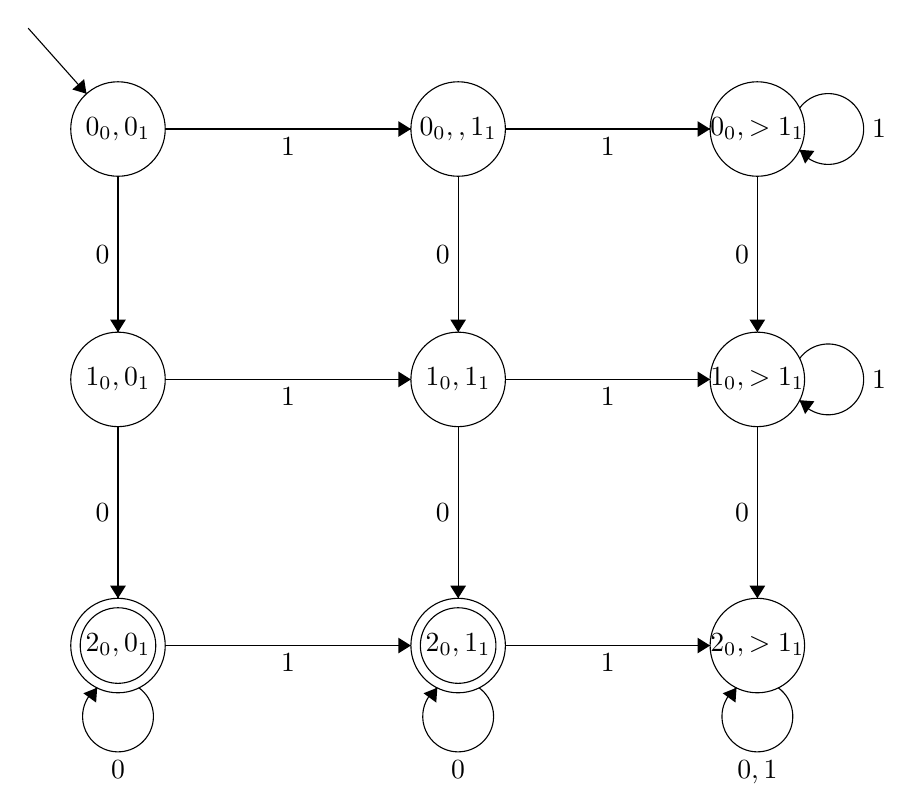
\begin{tikzpicture}[scale=0.2]
				\tikzstyle{every node}+=[inner sep=0pt]
				\draw [black] (12.4,-15.1) circle (3);
				\draw (12.4,-15.1) node {$0_0,0_1$};
				\draw [black] (12.4,-31) circle (3);
				\draw (12.4,-31) node {$1_0,0_1$};
				\draw [black] (12.4,-47.9) circle (3);
				\draw (12.4,-47.9) node {$2_0,0_1$};
				\draw [black] (12.4,-47.9) circle (2.4);
				\draw [black] (34,-15.1) circle (3);
				\draw (34,-15.1) node {$0_0,,1_1$};
				\draw [black] (53,-15.1) circle (3);
				\draw (53,-15.1) node {$0_0,>1_1$};
				\draw [black] (34,-31) circle (3);
				\draw (34,-31) node {$1_0,1_1$};
				\draw [black] (53,-31) circle (3);
				\draw (53,-31) node {$1_0,>1_1$};
				\draw [black] (34,-47.9) circle (3);
				\draw (34,-47.9) node {$2_0,1_1$};
				\draw [black] (34,-47.9) circle (2.4);
				\draw [black] (53,-47.9) circle (3);
				\draw (53,-47.9) node {$2_0,>1_1$};
				\draw [black] (6.7,-8.7) -- (10.4,-12.86);
				\fill [black] (10.4,-12.86) -- (10.25,-11.93) -- (9.5,-12.59);
				\draw [black] (12.4,-18.1) -- (12.4,-28);
				\fill [black] (12.4,-28) -- (12.9,-27.2) -- (11.9,-27.2);
				\draw (11.9,-23.05) node [left] {$0$};
				\draw [black] (15.4,-15.1) -- (31,-15.1);
				\fill [black] (31,-15.1) -- (30.2,-14.6) -- (30.2,-15.6);
				\draw (23.2,-15.6) node [below] {$1$};
				\draw [black] (37,-15.1) -- (50,-15.1);
				\fill [black] (50,-15.1) -- (49.2,-14.6) -- (49.2,-15.6);
				\draw (43.5,-15.6) node [below] {$1$};
				\draw [black] (15.4,-31) -- (31,-31);
				\fill [black] (31,-31) -- (30.2,-30.5) -- (30.2,-31.5);
				\draw (23.2,-31.5) node [below] {$1$};
				\draw [black] (37,-31) -- (50,-31);
				\fill [black] (50,-31) -- (49.2,-30.5) -- (49.2,-31.5);
				\draw (43.5,-31.5) node [below] {$1$};
				\draw [black] (15.4,-47.9) -- (31,-47.9);
				\fill [black] (31,-47.9) -- (30.2,-47.4) -- (30.2,-48.4);
				\draw (23.2,-48.4) node [below] {$1$};
				\draw [black] (37,-47.9) -- (50,-47.9);
				\fill [black] (50,-47.9) -- (49.2,-47.4) -- (49.2,-48.4);
				\draw (43.5,-48.4) node [below] {$1$};
				\draw [black] (12.4,-34) -- (12.4,-44.9);
				\fill [black] (12.4,-44.9) -- (12.9,-44.1) -- (11.9,-44.1);
				\draw (11.9,-39.45) node [left] {$0$};
				\draw [black] (34,-34) -- (34,-44.9);
				\fill [black] (34,-44.9) -- (34.5,-44.1) -- (33.5,-44.1);
				\draw (33.5,-39.45) node [left] {$0$};
				\draw [black] (53,-34) -- (53,-44.9);
				\fill [black] (53,-44.9) -- (53.5,-44.1) -- (52.5,-44.1);
				\draw (52.5,-39.45) node [left] {$0$};
				\draw [black] (53,-18.1) -- (53,-28);
				\fill [black] (53,-28) -- (53.5,-27.2) -- (52.5,-27.2);
				\draw (52.5,-23.05) node [left] {$0$};
				\draw [black] (34,-18.1) -- (34,-28);
				\fill [black] (34,-28) -- (34.5,-27.2) -- (33.5,-27.2);
				\draw (33.5,-23.05) node [left] {$0$};
				\draw [black] (13.723,-50.58) arc (54:-234:2.25);
				\draw (12.4,-55.15) node [below] {$0$};
				\fill [black] (11.08,-50.58) -- (10.2,-50.93) -- (11.01,-51.52);
				\draw [black] (35.323,-50.58) arc (54:-234:2.25);
				\draw (34,-55.15) node [below] {$0$};
				\fill [black] (32.68,-50.58) -- (31.8,-50.93) -- (32.61,-51.52);
				\draw [black] (54.323,-50.58) arc (54:-234:2.25);
				\draw (53,-55.15) node [below] {$0,1$};
				\fill [black] (51.68,-50.58) -- (50.8,-50.93) -- (51.61,-51.52);
				\draw [black] (55.68,-29.677) arc (144:-144:2.25);
				\draw (60.25,-31) node [right] {$1$};
				\fill [black] (55.68,-32.32) -- (56.03,-33.2) -- (56.62,-32.39);
				\draw [black] (55.68,-13.777) arc (144:-144:2.25);
				\draw (60.25,-15.1) node [right] {$1$};
				\fill [black] (55.68,-16.42) -- (56.03,-17.3) -- (56.62,-16.49);
			\end{tikzpicture}
		\end{align*}
	\end{enumerate}
\end{document}
